\documentclass[12pt, french]{article}

\usepackage{fancyhdr, fancybox, lastpage}
\usepackage[scr=rsfs]{mathalpha}
\usepackage[most]{tcolorbox}
\usepackage[a4paper, margin={0.3in, .75in}]{geometry}
\usepackage{wrapfig}
\pagestyle{fancy}
\renewcommand\headrulewidth{1pt}
\renewcommand\footrulewidth{1pt}
\fancyhf{}
\rhead{ \em{Zakaria Haouzan}}
\lhead[C]{\em{2ème année baccalauréat Sciences Physiques}}
\chead[C]{}
\rfoot[C]{}
\lfoot[R]{}
\cfoot[]{\em{Page \thepage / \pageref{LastPage}}}


\newtcolorbox{Box2}[2][]{
                lower separated=false,
                colback=white,
colframe=white!20!black,fonttitle=\bfseries,
colbacktitle=white!30!gray,
coltitle=black,
enhanced,
attach boxed title to top left={yshift=-0.1in,xshift=0.15in},
title=#2,#1}


\begin{document}
\begin{center}
   \shadowbox {\bf{ Noyau , énergie et masse }}
\end{center}


\vspace{-0.2cm}
$m(_0^1n)=1,00866u$ ; $m(_1^1p)=1,00728u$ ; $m(\beta)=5,48579.10^{-4}u$ ; $1MeV=1,6022.10^{-13}J$ ; Unité de masse atomique : $1u = 1,66055.10^{-27} kg=931,5MeV/c^2$ ; Constante d’Avogadro $N_A = 6,022.10^{23} mol^{-1}$ ;
%%_________________________Exercice ! :"_________________________Exercice
   \begin{Box2}{Exercice 1 :La désintégration d'un nucléide  }
La désintégration du nucléide $^{36}_{17}Cl$ donne naissance au nucléide $_{18}Ar$.
\begin{enumerate}
	\item Donner la composition du noyau 36
	\item Calculer en MeV l’énergie de liaison du noyau du chlore 36. Masse de Chlore 36 M(Cl) =35,9590 g/mol
\end{enumerate}
   \end{Box2}


%%_________________________Exercice !2 :"_________________________Exercice
\begin{Box2}{Exercice 2 :l’énergie de liaison}
%\begin{wrapfigure}{r}{0.22\textwidth}
  %\begin{center}
	  %\vspace{-0.6cm}
	%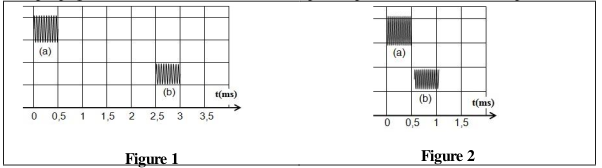
\includegraphics[width=0.22\textwidth]{./img/Ex2.png}
  %\end{center}
%\end{wrapfigure}
Masse du noyau du Radon 222 : 221,9703u , De la désintégration de l’Uranium 238 $^{238}_{92}U$ , résulte le Radon $_{86}Rn$ et des particules $\alpha$ et $\beta^-$.
	\begin{enumerate}
		\item Donner la composition du noyau $^{222}_{86}Rn$.
		\item  Calculer en (MeV) l’énergie de liaison du noyau $^{222}_{86}Rn$.
		\item  Déterminer le nombre de désintégration de type $\alpha$ et de type $\beta^-$ produites par cette transformation nucléaire
	\end{enumerate}
\end{Box2}


\begin{Box2}{Exercice 3 :l’énergie de liaison par nucléon }
Masse du noyau d’Uranium 238 : 238,00031 u , Masse du noyau du Plomb 206 : 205,92949u

Energie de liaison par nucléon du Plomb 206 :$\mathscr{E}(Pb) = 7,87$Mev/nucléon

Calculer l’énergie de liaison par nucléon de l’Uranium 238, et vérifier que le noyau $^{206}_{82}Pb$ est 238 plus stable que le noyau $^{238}_{92}U$


\end{Box2}


\begin{Box2}{Exercice 4 :La désintégration du noyau de cobalt }
La désintégration du noyau de cobalt $^{60}_{27}Co$ donne un noyau de nickel $_{28}Ni$et une particule X.

La masse du noyau $^{60}_{27}Co$: 59,91901 u , La masse du noyau $^{60}_{28}Ni$ : 59,91543 u.

L’énergie de liaison par nucléon du noyau $^{56}_{28}Ni$ : 8,64MeV/nucléon

\textbf{1. }Identifier la particule X, puis déterminer le type de désintégration du cobalt 60.

\textbf{2. } Calculer, en MeV, l’énergie libérée $E_{lib}$ au cours de cette désintégration.

\textbf{3. }Déterminer, en MeV/nucléon, l’énergie de liaison par nucléon $\mathscr{E}$ du noyau $^{60}_{28}Ni$ , puis déduire parmi les deux noyaux $^{60}_{28}Ni$ et $^{56}_{28}Ni$, lequel est le plus stable.

\end{Box2}
%\vspace{2cm}

\begin{center}
   \Large{ \em{Exercices Supplémentaires}}
\end{center}



\begin{Box2}{Exercice 5 :Application de la radioactivité dans la médecine }
L’histoire de la médecine nucléaire a toujours été lié au progrès de la physique nucléaire. Dans
plusieurs cas la médecine nucléaire consiste à injecter des produits radioactifs dans le corps humain
pour diagnostiquer et remédier à la maladie. L’isotope $^{99}_{43}Tc$ du technétium est parmi les noyaux les
plus utilisés dans le domaine de la médecine à cause de sa durée de vie courte, ses effets radioactifs
minimal, son cout très bas, et la facilite de sa mise à disponibilité des médecins.
Cet exercice a pour but l’étude d’une des utilisations du technétium dans le domaine médical.
\begin{itemize}
	\item Énergie de liaison : 

		$E_L(^{99}_{43}Tc) = 852,53MeV$ ; $E_L(^{97}_{43}Tc) = 836,28MeV$

	\item La demi-vie du technétium $^{99}_{43}Tc$ est $t_{1/2}$ = 6h.
\end{itemize}

\textbf{1. }Les noyaux $_{43}Tc$ et $_{43}Tc$ sont deux isotopes de Technétium.

\textbf{1.1. }Donner la composition de l’isotope $^{99}_{43}Tc$ du noyau de technétium.

\textbf{1.2. }Quel est le noyau le plus stable ? Justifier votre réponse.

\textbf{1.3. }Le technétium $^{99}_{43}Tc$ est produit par la désintégration d’un noyau du molybdène $^{99}_{42}Mo$ , préciser le type de la désintégration
radioactive.

\textbf{2. }Le technétium $^{99}_{43}Tc$ est utilisé dans le domaine de la radiologie, on injecte à un malade une dose de technétium $^{99}_{43}Tc$ puis on prend les cliches de ces os.

À l’instant $t_0=0$ on injecte a un patient une dose d’activité radioactive $a_0 = 5.10^8Bq$, puis on prend
une image-radio des os à l’instant t1, l’activité radioactive devient $a_1 = 0,6a_0$.

\textbf{2.1 }Vérifier que la valeur de la constante d’activité radioactive du technétium $^{99}_{43}Tc$ est $\lambda = 3,21.10^{-5} s^{-1}$.

\textbf{2.2 }Déterminer la valeur $N_0$, le nombre de noyaux injectés dans le corps à l’instant $t_0 =0$.
\textbf{2.3 }Déterminer en heure (h) la valeur de t.

\end{Box2}

\begin{Box2}{Exercice 6 :La radioactivité dans le tabac}
Le tabac est l’une des causes principales du cancer du poumon, cette cause est dû essentiellement a
des effets chimiques et peu de rayonnement nucléaire car le tabac contient l’isotope $^{210}_{84}Po$ de l’élément polonium radioactif	

\begin{center}
\begin{tabular}{ |c|c|c|c|c|c| }
	\hline
 Le noyau  & Thallium        & Hélium       & Plomb & Bismuth & Polonium\\\hline 
 Le symbole & $^{206}_{81}Tl$ & $^{4}_{2}He$& $^{206}_{82}Pb$ & $^{209}_{83}Bi$&$^{210}_{84}Po$\\\hline
Masse du noyau (u)& 205,9317 & 4,0015 & 205,9295 &208,9348 & 209,9368\\\hline
$t_{1/2}$ du $^{210}_{84}Po$ & & & & & 138jours\\\hline

\end{tabular}
\end{center}
\textbf{1. }Le noyau du polonium $^{210}_{84}Po$ est radioactif $\alpha$. Écrire l’équation de désintégration du noyau du
polonium en déterminant le noyau fils.

\textbf{2. }Vérifier que la constante radioactive du noyau polonium $^{210}_{84}Po$ est $\lambda = 5,81.10^{-8}s^{-1}$.

\textbf{3. }On dispose d’un échantillon radioactif du polonium $^{210}_{84}Po$ son activité à l’instant t est $a_0 = 10^{-1} Bq$

\textbf{3.1. }Déterminer la valeur de N le nombre de noyaux de polonium $^{210}_{84}Po$ dans l’échantillon à l’instant t .

\textbf{3.2. }Calculer en MeV, la valeur de l’énergie libérée ELibérée durant la désintégration de N noyaux de polonium $^{210}_{84}Po$


\end{Box2}
\end{document}
